\documentclass{report}
\usepackage{graphicx, chemformula, titlesec,pdfpages}
\usepackage[a4paper, portrait, margin=1in]{geometry}
\usepackage[table,xcdraw]{xcolor}
\title{Accreditation course in radiation protection - Radiation Protection Officer – Dispersible radioactive substances level D (TMS-VRS D)}
\date{September 2025}
\begin{document}
\maketitle
\tableofcontents
%-------------------------------------------------------------------------------------------------------------------------------------------------------------------------------------------------------------------------------------------------------------------------------------------------------------------------------------%x
\part{Quick reference handbook}
\chapter{Radioactive decay}
\textbf{$\alpha$ decay}: Occurs when the nucleus is unstable, due to being too big. The parent atom $\ch{^{A}_{Z}X}$ gets split into a daughter atom $\ch{^{A-4}_{Z-2}Y}$ and an alpha particle $\ch{^{4}_{2}a}$.\\\\
\textbf{$\beta^{-}$ decay}: Occurs when the nucleus is unstable, due to having an excess of neutrons. The parent atom $\ch{^{A}_{Z}X}$ gets split into a daughter atom $\ch{^{A}_{Z+1}Y}$, a beta particle $\ch{^{0}_{-1}e^{-}}$, and an anti-neutrino $\overline{v}_e$.\\\\
\textbf{$\beta^{+}$ decay}: Occurs when the nucleus is unstable, due to having an excess of protons. The parent atom $\ch{^{A}_{Z}X}$ gets split into a daughter atom $\ch{^{A}_{Z+1}Y}$, a positron $\ch{^{0}_{+1}e^{+}}$, and a neutrino $v$. After a number of interactions, the positron $\beta{+}$ unites with an electron and converts its entire mass to energy. This annihilation produces 511 keV.\\\\
\textbf{Electron capture}: The nucleus absorbs an electron from the electron cloud (usually from shell K -innermost). The parent atom $\ch{^{A}_{Z}X}$ absorbs an electron $\ch{^{0}_{-1}e^{-}}$, and gets split into a daughter atom $\ch{^{A}_{Z-1}Y}$, and a neutrino $v$.\\\\
\textbf{Gamma decay ($\gamma$)} Occurs when the atom is excited. The parent atom $\ch{^{A}_{Z}X*}$ gets excited and produces a daughter particle $\ch{^{A}_{Z}X}$ and a gamma ray $\gamma^{1}$. Internal conversion may occur (direct transsfer of the energy of the nucleus to an electron).
%--------------------------------------------------------------------------------------------------------------------------------------------------------------------------------------------------------------------------------------------------------------------------------------------------------------------------%
\chapter{Formulas}
\section{Activity determination}
\[A(t) = A(0) \cdot (\frac{1}{2})^{\frac{t}{T_{1/2}}}\]
\textbf{Precise determination with a formula for the half-life using half-life}. All time units must be in the same unit.\\
\[\frac{dN(t)}{dt}=-\lambda\cdot N(t);\ A(t) = A(0)\cdot e^{-\lambda t}\]
\textbf{Precise determination with a formula for the half-life using decay constant ($\lambda$)}. All time units must be in the same unit.\\

\section{Shielding}
\[g \approx 2\cdot10^{-4}\cdot Z\cdot E_{\beta,max}\]
\textbf{Approximation of the energy converted to Bremsstrahlung}. Where $Z$ is the atomic number of the shielding material\\
\[R_{\beta,\ in\ material} = \frac{R_{\beta,\ in\ water} = 0.5 E_{\beta,max}}{\rho_{material}}\]
\textbf{Range of $\beta$ particle in a specific material}. For water and tissue, $\rho$ can be estimated to be 1 g/cm³. $E_{\beta,max}$ is expressed in MeV.\\
\[I(d) = I(0)\cdot B\cdot(\frac{1}{2})^{\frac{d}{d_{1/2}}}\]
\textbf{Shielding of $\gamma$ radiation using half distance}. Buildup factor (P60) may be ignored. All distance units must be in the same unit.\\
\[I(d) = I(0)\cdot e^{-\mu_{linear} d}; \mu_{mass} = \mu_{linear}\cdot\rho_{material}^{-1}\]
\textbf{Shielding of $\gamma$ radiation using linear attenuation coefficient}. Above 500keV, $\mu_{mass\ water}\approx\mu_{mass\ concrete}$.\\

\section{Dose determination}
\[H_T = W_R \cdot D\]
\textbf{Equivalent dose}. $W_R$ is the radiation weighting factor: 1x for $\beta$ and $\gamma$, 20x for $\alpha$, and 2-20x for $N_0$. D is the absorbed dose over tissue of organ (Gy).\\
\[E = \sum (W_T \cdot H_T)\]
\textbf{Effective dose}. $W_T$ is the tissue weighting factor (P64). \\
\[E(50) = e(50)\cdot A\]
\textbf{Committed effective dose (Sv)}. e(50) is the committed effective dose coefficient (Sv$\cdot$Bq$^{-1}$).\\
\[\cdot H*(10) = h(10)\cdot\frac{A}{r²}\]
\textbf{Inverse square law}. The activity must be in MBq, the distance in m, and the result in $\mu$Sv/h\\
\[X\]
\textbf{}\\

\section{Measurement}
\[rel. error = \frac{\sqrt{N}}{N} = \frac{1}{\sqrt{N}}\]
\textbf{Relative error}. $N$ is the number of counted pulses, $\sqrt{N} is the counting error$\\
\[\epsilon = \frac{R}{A}\]
\textbf{Efficiency}, where R is the counting rate in units of per second, and A is the activity in Bq.\\
%--------------------------------------------------------------------------------------------------------------------------------------------------------------------------------------------------------------------------------------------------------------------------------------------------------------------------%
\chapter{Useful information}
\begin{figure}
    \centering
    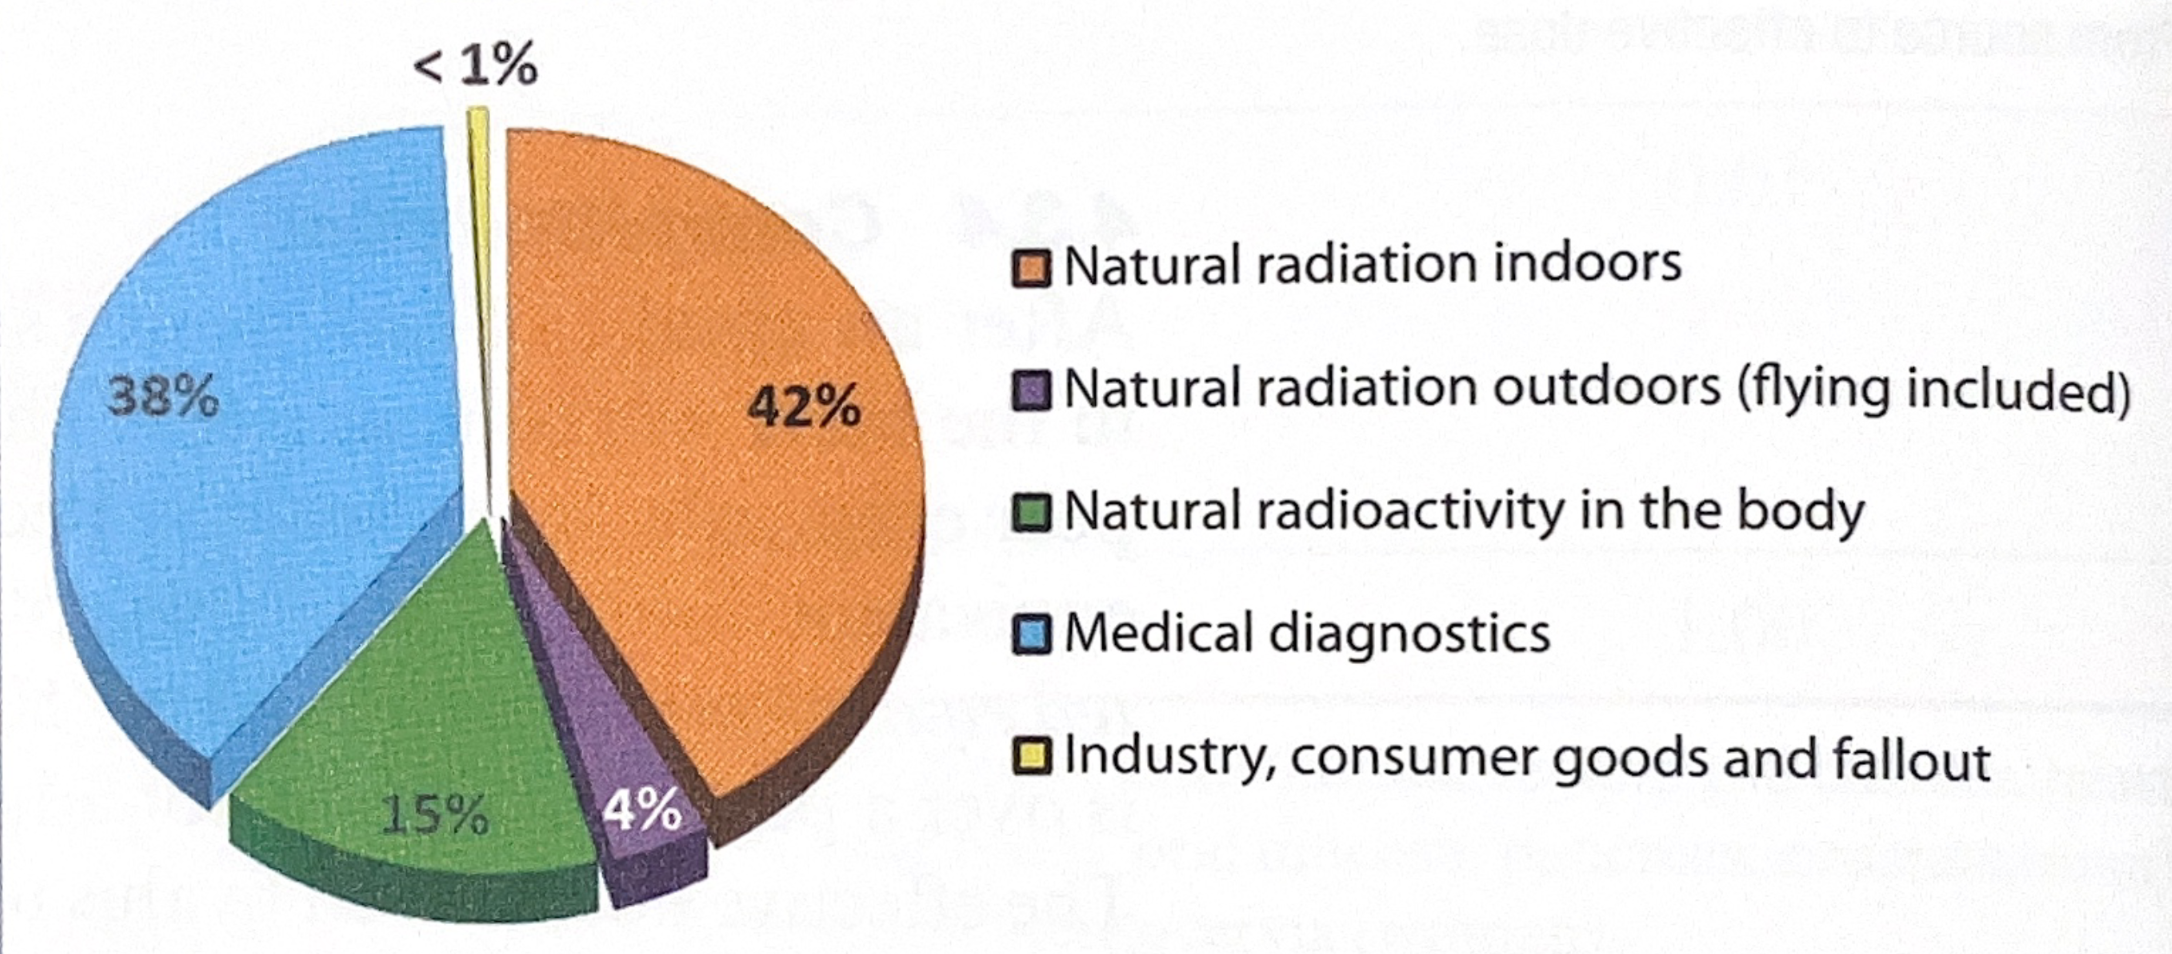
\includegraphics[width=0.5\linewidth]{Normal_dose.png}
    \caption{Contributions to the dose for a member of the public in the Netherlands}
    \label{fig:placeholder}
\end{figure}
\begin{table}[ht]
\caption{Detectors and their usual applications}
\label{detect}
\begin{tabular}{lll}
\hline
 & $\beta$ emitters & Photon radiation \\ \hline
\textbf{Ionisation detectors} &  &  \\
GM Tube (thin window) & Contamination & Contamination \\
GM Tube (thick window) & - & Dose rate \\
Proportional counter (thin window, xenon filled) & Large area contamination & Large area contamination \\for low-energy photons \\
Germanium semiconductor & - & Accurate spectrum \\ \hline
\textbf{Scintillation detectors} &  &  \\
Nal(Tl) & - & \begin{tabular}[c]{@{}l@{}}Contamination\\ Simple spectrum\\ Dose rate\end{tabular} \\
Andthracene or ZnS & Contamination & Contamination \\
TLD & Personal dosimeter & Personal dosimeter \\
 &  & 
\end{tabular}
\end{table}
%----------------------------------%
\begin{table}[ht]
\caption{Dose limits}
\label{doses}
\begin{tabular}{llll}
\rowcolor[HTML]{343434} 
\multicolumn{1}{l|}{\cellcolor[HTML]{343434}{\color[HTML]{FFFFFF} \textbf{Group}}} & \multicolumn{1}{l|}{\cellcolor[HTML]{343434}{\color[HTML]{FFFFFF} \textbf{\begin{tabular}[c]{@{}l@{}}Effective dose [mSv/y]\end{tabular}}}} & \multicolumn{2}{l}{\cellcolor[HTML]{343434}{\color[HTML]{FFFFFF} \textbf{\begin{tabular}[c]{@{}l@{}}Equivalent dose [mSv/y]\end{tabular}}}} \\
\rowcolor[HTML]{C0C0C0} & \multicolumn{1}{l|}{\cellcolor[HTML]{C0C0C0}{\color[HTML]{333333} Total body}} & \multicolumn{1}{l|}{\cellcolor[HTML]{C0C0C0}{\color[HTML]{333333} Eye lens}} & {\color[HTML]{333333} Skin \& extremities} \\ \hline
\textbf{Category A} & 20 & 20 & 500 \\
\textbf{\begin{tabular}[c]{@{}l@{}}Category B\\ Exposed pupils and students\\ Those between 16 and 18\end{tabular}} & 6 & 15 & 150 \\
\textbf{\begin{tabular}[c]{@{}l@{}}Category C\\ ``Non-exposed employees''\end{tabular}} & 1 & 15 & 50 \\
\textbf{Pregnant employees} & \multicolumn{3}{l}{Maximum 1 mSv equiv to abdomen from announcement to birth.} \\
\textbf{\begin{tabular}[c]{@{}l@{}}Members of the public\\ Excluding patients\end{tabular}} & 1 & 15 & 50
\end{tabular}
\end{table}































%\[X\]
%\textbf{}\\
%-------------------------------------------------------------------------------------------------------------------------------------------------------------------------------------------------------------------------------------------------------------------------------------------------------------------------------------%
\setcounter{page}{1}\part{Classes}
\chapter{Physics 1}%-------------------------------------------------------------------------------------------------------------------------------------------------------------------------------------------------------------------------------------------------------------------------------------------------------------------------------------%
\section{Structure of an atom}
An atom of X element has Z number of protons, N number of neutrons [n(0)], and a mass (A) of Z+N. \\
An element can be expressed as $\ch{^{A}_{Z}X}$ \par.
%-------------------------------------------------------------------------------------------------------------------------------------------------------------------------------------------------------------------------------------------------------------------------------------------------------------------------------------%
\section{Radioactive decay}
Decay may occur due to:
 \begin{enumerate}
	\item Too many protons
	\item Too many neutrons
	\item Too many neutrons and protons
	\item Energetically excited state
\end{enumerate}
The chart of nucleides expresses in black the stable nuclei and in white the unstable nuclei. Isobars have the same mass (A), and isotopes have the same number of P+ (Z).
%-------------------------------------------------------------------------------------------------------------------------------------------------------------------------------------------------------------------------------------------------------------------------------------------------------------------------------------%
\section{Ionizing radiation}
Radiation is energy released as electromagnetic waves or particles. \\
Ionisation means removing electrons from the electron cloud of the atom. \\
Ionising radiation can consist of:
 \begin{enumerate}
	\item Particle radiation (with high energy)
	 \begin{enumerate}
		\item Alpha decay
		\item Beta decay
		\item Electron capture
		\item Positron emission
	\end{enumerate}
	 \item Electromagnetic radiation (with high energy)
	 \begin{enumerate}
		\item Isomeric transition (gamma emission)
	\end{enumerate}	 
\end{enumerate}
The radiation type that occurs can be seen on the chart of nucleides (see slide 10). 
\subsubsection{Alpha decay ($\alpha$)}
Occurs when the nucleus is unstable, due to being too big.\\
The parent atom $\ch{^{A}_{Z}X}$ gets split into a daughter atom $\ch{^{A-4}_{Z-2}Y}$ and an alpha particle $\ch{^{4}_{2}a}$.
\subsubsection{Beta decay ($\beta$)}
Occurs when the nucleus is unstable, due to having an excess of n.\\
The parent atom $\ch{^{A}_{Z}X}$ gets split into a daughter atom $\ch{^{A}_{Z+1}Y}$, a beta particle $\ch{^{0}_{-1}e^{-}}$, and an anti-neutrino $\overline{v}_e$.
\subsubsection{Electron capture (E.C. or $\epsilon$)}
Occurs when the nucleus is unstable, due to having an excess of p.\\
The parent atom $\ch{^{A}_{Z}X}$ absorbs an electron $\ch{^{0}_{-1}e^{-}}$, and gets split into a daughter atom $\ch{^{A}_{Z-1}Y}$, and a neutrino $v$.
If the hole is filled by an outer shell electron, X-rays are emmitted.
[...]
\subsubsection{Positron emission ($\beta^{+})$}
Occurs when the nucleus is unstable, due to having an excess of p.\\
The parent atom $\ch{^{A}_{Z}X}$ gets split into a daughter atom $\ch{^{A}_{Z+1}Y}$, a positron $\ch{^{0}_{+1}e^{+}}$, and a neutrino $v$.
After a number of interactions, the positron unites with an electron and converts its entire mass to energy. This annihilation produces 511 keV.
\subsubsection{Gamma decay ($\gamma$)}
Occurs when the atom is excited.\\
The parent atom $\ch{^{A}_{Z}X*}$ gets excited and produces a daughter particle $\ch{^{A}_{Z}X}$ and a gamma ray $\gamma^{1}$.
%-------------------------------------------------------------------------------------------------------------------------------------------------------------------------------------------------------------------------------------------------------------------------------------------------------------------------------------%
\section{Activity}
\subsection{Unit of activity (A)}
The unit of activity is the Becquerel (Bq). 1 Bq = 1 disintegration per second.
The specific activity is the activity per mass (Bq/g)
The old unit was Curie (Ci), equivalent to $3.7·10^{10}Bq$
 \subsection{Decay law}
 Decay is a random process. 
Activity is proportional to the number of nuclei and the decay constant $\lambda (s^{-1})$:
\[ A = -\frac{dN}{dt} = \lambda N \]
The half life is the number of seconds that it takes to decay half of all nuclei present:
\[ t_{1/2} = -\frac{ln2}{\lambda} = \frac{0.693}{\lambda} \]
The activity ($A_t$) on time (t) can be approximated as:
\[ A_{t} = A_0 * e^{-\frac{t}{t_{1/2}}*ln(2)} \]
\[ A_{t} = A_0 * \frac{1}{2}^{-\frac{t}{t_{1/2}}} \]
%-------------------------------------------------------------------------------------------------------------------------------------------------------------------------------------------------------------------------------------------------------------------------------------------------------------------------------------%
\section{Electromagnetic radiation}
Electromagnetic radiation is non-material. \\
The smaller the wavelength, the higher the frequency, and the higher the energy.
\[ \lambda = \frac{c}{v} \]
\[E = \frac{hc}{\lambda} = h*v \]

\subsection{Generation of X-rays}
X-rays happen when high energy atoms are slowed down by matter. An atom is bombarded by electrons. When an electron hits another electron, a hole is formed. This is then filled by an electron from the electron shell, which releases energy. Three situations can occur: 
 \begin{enumerate}
	\item The electron can hit the nucleus, which produces the maximum energy.
	\item The electron can have a close interaction, which produces moderate energy.
	\item The electron can have a distant interaction, which prouces low energy.
\end{enumerate}
The X-ray tube produces X-rays. It depends on the electron energy (regulated by the tube voltage), and the anode material (usually tungsten). <1\% of energy is converted to X-rays, and the rest is heat. 
The X-ray tube has a spectrum of emission, called the Spectrum Bremsstrahlung.
In an X-ray spectrum there's always peaks. Those are called the characteristic X-rays, and they depend on the material. X-rays can be filtered or unfiltered. This reduces the amount of X-rays in the areas that aren't of interest. The filter affects the X-rays differently depending on the material it's made out of.

\subsection{Interaction of radiation with matter}
Gamma and X-rays can interact with matter in the following ways:
 \begin{enumerate}
	\item Classic scattering (mainly non-ionising radiation)
	\item Photo effect
	\item Compton effect
	\item Pair production
\end{enumerate}
Which method occurs depends on the photon energy and the atomic number (see slide 61)
\subsubsection{Classic scattering}
Also called elastic, coherent or Rayleigh scattering.
Gamma energy remains unchanged, but the direction of the photon may change. It is important at low $E_{\lambda}$

\subsubsection{Photo effect}
The photon knocks an electron out of its orbit. The electron has binding energy, so the resulting energy is minimal. It goes up to 0.5MeV. The chance is roughly proportional to $Z^4$, and it produces characteristic X-rays.

\subsubsection{Compton effect}
The dominant effect at higher energies. Depends on the material.
The photon is scattered at weakly bound electrons, transferring partly the energy to the electron. However, it continues and may hit another electron. It can go through the material, with less energy that it came in.
The degree of energy transfer depends on the scatter angle. The maximal energy will be at 180ª, and the minimal energy at 0º. With a portable X-ray tube it's better to have it below the bed, as it's shielded, and most of the backscatter will go to the rear.

\subsubsection{Pair production}
Near the nucleus, the photon can create both an electron and a positron, if it has enough energy. This usually results in an annihilation, usually outside of the atom, creating 2 511keV photons, at 180º from each other. This can only occur at energies of over 1.022MeV (mass of the electron + positron). 


\chapter{Physics 2}%-------------------------------------------------------------------------------------------------------------------------------------------------------------------------------------------------------------------------------------------------------------------------------------------------------------------------------------%
\section{Interaction of charged particles with matter}
Photons do not experience energy loss per distance. However, charged particles do. There is a certain amount of energy loss per cm (LET: Linear Energy Transfer), or Stopping Power. Alpha particles have a high stopping power, as they lose a lot of energy at a short distance.\\
The range is the maximum distance that charged particles can travel in matter. It depends on the type of charged particle, the energy of the charged particle, and the density of the material. Not every electron has the same speed, as the energy is distributed unequally and randomly between the electron and the neutrino. The mean energy is lower than the 50\% of the range. \\
Rule of thumb (produces an overestimation) for $\beta$ with E > 0.6 MeV:
\[ R (cm) * \rho (\frac{g}{cm³} )= 0.5\ E_{\beta,max} (MeV) \]
Soft tissue is very equivalent to water, and thus can be approximated to a density of 1. Air is around 1000 times higher.

\subsection{Interaction of $\alpha$ particles with matter}
Due to the interaction with the electrons of atoms (ionizations and excitations), the energy of an $\alpha$ particle decreases. It disposes of its energy linearly along a straight path. The range/pathway depends on the energy of the radiation and the density of the material\\
Alpha particles have a high stopping power. They lose a lot of energy at a short distance (small range, thick track). They are unable to pass the epidermis, but they are very dangerous if ingested. \\

\subsection{Interaction of protons with matter}
Protons behave like $\alpha$ particles, but they can be directed to deposit most of their energy at a specific point (Bragg peak). The Bragg peak can be manipulated with the energy.

\subsection{}


\subsection{Shielding from ionizing radiation}
Shielding for particles only needs to be as thick as the maximal range. However, for photons, you the shielding needs to be as thick as deemed reasonably safe. \\
The $\gamma$-photon pathway is much longer than the $\beta$-particle, which is longer than the $\alpha$-particle pathway.
\subsubsection{Alpha}
For $\alpha$ particles, barely any shielding is necessary. 
\subsubsection{Beta}
For $\beta$ particles, the rule of thumb can be applied. Shielding materials with a low Z-value cause less Bremsstrahlung. Such materials are Perspex or aluminum (mostly Perspex, as it's see-through, and has an even lower Z-value). Bremsstrahlung causes a loss of energy, which is released as a photon, usually in the X-ray range. $\beta$ emmitters are usually stored in a perspex container in a lead container. Perspex is often used a a mimic for tissue.
\subsubsection{Gamma}
For $\gamma$ and X-rays, the material cannot stop them entirely but rather attenuate them. It depends on the energy of the radiation, and the density of the material (or rather Z value, the highest Z-value attenuates the most). The attenuation can be calculated with:
\[  I_d = I_0\ e^{-\mu d}   \]
Where d is the thickness of the material and $\mu$ is the attenuation coefficient. After $d_{1/2}$, the photon intensity is halved:
\[  d_{1/2} = \frac{ln2}{\mu}  \]
Transmission is the ratio between the original intensity and the dampened intensity.
\[  T = \frac{I_d}{I_0}	 \]

\subsection{Inverse square law}
Electromagnetic radiation is a Newtonian form of radiation, which means that it decreases in intensity by the square of the distance. This is because the intensity is the number of photons/sm², and the surface of a sphere increases with the square of the radius.

\section{Dose}
\subsection{Definition of dose}
An absorbed dose (D) is the absorbed energy per mass of matter. We use the Gray (Gy), equivalent to 1 Joule/kg.
\subsection{Calculation of a $\gamma$ dose rate}
\[ H = \frac{h(10)A}{r^2} \]
Where h(10) is the ambience dose equivalent rate/source constant, H is the dose rate, A is the activity, and r is the distance.\\
The h(10) is exclusive for nucleides with gamma emission. There's tables that can be used.
\subsection{Rules of thumb}

\subsubsection{$\beta$ radiation}
The source of an A MBq source that emits a $\beta$ particle of E MeV per decay event at 10 cm is
\[ H_{skin} = 1000A (\frac{\mu Sv}{h} \]

\subsubsection{$\gamma$ radiation}
The source of an A MBq source that emits a $\gamma$ photon of E MeV per decay event at 30 cm is
\[ H = 2A (\frac{\mu Sv}{h} \]

\subsection{Dose reduction}
 \begin{enumerate}
	\item Time $\rightarrow$ Work fast
	\item Distance $\rightarrow$ Stay away
	\item Shielding $\rightarrow$ Use shielding
	\item Activity $\rightarrow$ Use the minimum needed
\end{enumerate}

\subsection{Buildup factor}
The attenuation law assumes a narrow beam. However, that's not correct. Depending on the shielding material, there may be a lot of backscatter, which amplifies the radiation after the shielding. The build-up factor depends on the energy and the material, and it may need additional shielding to compensate. The buildup factor can be considerable, commonly factor 2-4, but even goes higher than 100.

\subsection{Dose and biology}
\begin{table}[]
\begin{tabular}{llll}
Quantity        & Symbol & Unit         & Type       \\
Absorbed dose   & D      & Gray (Gy)    & Physical   \\
Equivalent dose & $H_T$    & Sievert (Sv) & Biological (Specific part) \\
Effective dose  & E      & Sievert (Sv) & Biological (Whole body)
\end{tabular}
\end{table}

\subsubsection{Equivalent dose}
The seriousness of biological tissue damage is also determined by the way that energy is disposed. It depends on the kind of radiation. $\alpha$ radiation has more ionizations per path length, so it does more damage than $\beta$ or $\gamma$.
\[ H_T = D * W_R\]
Where $W_R$ is the radiation weighting factor, and D is the absorbed dose in Gray

\begin{table}[]
\begin{tabular}{ll}
Type of radiation & $W_R$    \\
$\beta$             & 1      \\
$\gamma$            & 1      \\
X-ray             & 1      \\
n                 & 5-20   \\
p                 & 1.1-10 \\
$\alpha$            & 20    
\end{tabular}
\end{table}

\subsubsection{Effective dose}
It is a quantity used for comparison of risks. The effective dose is the radiation dose needed in homogenous total body irradiation to obtain the same risk.
\[ \sum_{T}^{}H_T\cdot W_T \]
Where $H_T$ is the equivalent dose and $W_T$ is the tissue weighting factor (See Table 5.2 in the book). $W_T$ depends on the rate of division of the cells in each organ.

\subsubsection{Dose Conversion Coefficients}
To calculate the effective (committed = internal) dose after contamination (ingestion) with radionucleides, the following formula is used:
\[ E_{committed} = A*e_{50}\]
E(50) is the effective dose received over 50 years after intake, and it depends on the chemical form, way of intake, and sometimes disease of the patient. The e(50) or DCC or $e_{inh/ing}$ is a coefficient that can be looked up on tables.

To calculate the effective dose after skin contamination, e(50) (Sv/Bq) and $DCC_{skin}$ (mSv/s per kBq/cm²) are used for contamination, h(10) is used for irradiation ($\mu$ Sv/h per MBq/m²)

\chapter{Measuring methods}The purpose of measuring is to determine the type of radiation, the activity, the energy of the radiation, or the (effective) dose or dose rate.
\section{Principles of radiation detection}
\begin{table}[]
\begin{tabular}{lll}
Principle of operation & Detector material                                                        & Detector type                                                              \\
Electrical charge      & \begin{tabular}[c]{@{}l@{}}Gas\\ Solid state\end{tabular}                & \begin{tabular}[c]{@{}l@{}}Gas-filled\\ Semiconductor\end{tabular}         \\
Luminescence           & \begin{tabular}[c]{@{}l@{}}Solid/liquid state\\ Solid state\end{tabular} & \begin{tabular}[c]{@{}l@{}}Scintillation\\ Thermoluminescence\end{tabular} \\
Chemical reaction      & Photographic emulsion                                                    & Densitometer                                                               \\
Warmth                 & Solid/liquid state                                                       & Calorimeter                                                                \\
Activation             & Solid state                                                              & Activation dose meter                                                     
\end{tabular}
\end{table}

\section{Ionization/Electric charge}
\subsection{Gas-filled detectors}
Gas-filled detectors have a closed tube that contain air or another gas. When radiation enters the tube, ionization occurs. The walls of the detector have a voltage between them, which separates the ions, and this can be measured through the current. The current is proportional to the primary electron-ion pairs, which is proportional to the absorbed amount of energy. However, these detectors have a a recombination region (Applied voltage < Saturation voltage), in which they can work. Above the saturation voltage, there's the saturation region, in which the detector can't detect more because all formed ion pairs can reach the electrodes, and cannot recombinate. They consist of a tube with very thin membranes at the end (protected by a mesh or bars).\\

\subsubsection{Ionization chamber}
They produce very small electrical signals. They aren't used in pulse mode to detect indiviual counts, but rather used for radiation intensity. They are most suited to detect radiation with high energy deposition ($\alpha$ or $\beta$), or with high energy, but it's not efficient for $\gamma$ rays. It can be used as a dose calibrator to determine the amount of radioactivity of a known radioisotope.

\subsubsection{Proportional counter region}
At sufficiently high voltage, the accelerated primary electrons have enough energy to cause ionization themselves and form secondary electron pairs (cascade).\\
The proportional counter uses the proportional counter region. It produces larger electrical signals than the ionization chamber, so it is used in pulse mode to detect individual counts. The electrical signal is proportional to the amount of deposited energy, so it can be used for energy selective counting. It's most suited to detect radiation with high energy deposition ($\alpha$ and $\beta$), and though it can detect $\gamma$, it's not as efficient. It can be used as a contamination monitor.

\subsubsection{Geiger-Müller region}
Similar to the proportional counter region, but even more. This is called the avalanche. At high voltage, emission photons are created, which can interact with gas, creating even more electron-ion pairs. The avalanche is stopped when a large number of 'slow' positive ions reduces the effective voltage, and the electrical charge becomes independent of absorbed energy.\\
The Geiger-Müller counter uses the Geiger-Müller region. It produces larger electrical signals that can be easily measured with low cost electronics, so they are used in pulse mode. The electrical signal is independent of absorbed energy, so it's not used for energy-selective counting. It's inefficient for $\gamma$ rays, but it's more sensitive than the ionization chamber and the proportional counters. They are used as survey monitors.

\subsection{Semiconductors}
They work in a similar way to the gas-filled detectors, but they're more efficient for X- and $\gamma$-rays, given their higher stopping power. The energy needed to create a single electron-ion pair is much lower than for air, so a larger electrical signal is produced.\\
Individual counts can be measured with a very high energy resolution, which produces an energy spectrum, which is a 'fingerprint' that is used to identify radio-isotopes.\\
In order to suppress noise they must be cooled, so they are immovile and very heavy.

\section{Luminescence}
\subsection{Scintillation}
They work through scintillations. This means that a photon is released in the UV or visible-light range when an excited electron returns to its ground state. The produced amount of light is proportional to the amount of energy. But this energy can be very small, so a photomultiplier tube is used by converting scintillation light to pulses of electrical current. The most common cathode is sodium iodide, or not as commonly, another salt. Radiation enters the crystal, and photons are released as a result.\\
Solid materials can be used, such as NaI or CsI (for $\gamma$ radiation), or anthracene or stilbene (plastics, used for $\alpha$ and $\beta$ radiation). Organic liquid materials can also be used to detect $\alpha$ or $\beta$ radiation (a small amount of sample is put in the liquid), and it's best used for low-energy sources, as it's often the only way to check for contamination (with swipe or smear tests).\\
Scintillation can also be used to identify materiials, although they have a lower resolution than semiconductors.

\subsection{Thermoluminescence}
It is often used in personal dosimeters. The thermoluminescent detector is made from a material that can emit photons upon heating after exposure to ionizing radiation. Therefore, it 'captures' radiation, and releases it when it's heated.

\section{Efficiency}
No detector is 100\% efficient. This is because even if the detector was perfect, you'd only be measuring by one side. The measurement efficiency depends on detector efficiency, geometric efficiency, the source, and the absorption between the source and the detector. The efficiency can be determined by measuring a source with known activity.
\[ \epsilon = \frac{R_{net}}{A} = \frac{R_{gross}-R_{background}}{A}\]
Where R<A, R being the count rate, and A being the actual activity. 

\section{Counting statistics}


\chapter{Biological Effects}\section{Effects of radiation on cells}
Everything in the cell is a possible target. However, the biggest risk is the nucleus, and its DNA. This is because it can create DNA damage, such as base damage, cross-links, single/double strand breaks. In oncology, double strand breaks are needed to treat cancer. 1Gy of LET X-rays produces 1000 single-strand breaks, 40 double-strand breaks and 1000 altered bases.

\subsection{DNA repair}
Cells have a lot of repair mechanisms. Double-stranded breaks can cause many errors due to non-homologous end-joining. NHEJ cuts corners for the sake of speed. Single-strand breaks are easily repaired, in a couple of minutes after irradiation, 80\% of breaks are repaired. Double-strand breaks take much longer, taking hours for the same 80\% of breaks being repaired. 

\subsection{Stochastic effects}
Chance is proportionally related to the dose. There's no threshold, any exposure is any damage. It can cause cancer or congenital defects. There may be a latency period. This is based on the multiple hit theory (multiple 'hits' are needed to cause cancer). The multiple hit theory says that multiple genetic changes are necessary. Oncogenes (such as Ras) are needed to quickly proliferate cells. Tumour supressor genes (such as p53 or RB1) are needed to prevent mutated cells from dividing. DNA-repair genes (such as HNPCC or BRCA) are needed to to repair the DNA. Leukemia is a more immediate form of cancer (around 10-20 years), but most other forms of cancer take at least 15 years. \\
However, electromagnetic radiation usually only makes around 5-7\% of the carcinogenic factors. This also includes the sun's radiation, radon gas from working inside (radon is formed in the same rocks that are used to make buildings). Cancer is a multi-factorial risk, so it's difficult to tell the cause of the cancer. However, risks can be estimated by having large groups of exposed and non-exposed individuals, knowing the exact dose everyone received, and having a big difference with background radiation. One example of research was the one done after Hiroshima and Nagasaki. They had over 85k subjects in the cohort, and it has been running since the atomic bombs. The subjects get questionnaires, medical checkups, etc. yearly. Using the position where everyone was in the city when the bombs hit, the dose was estimated, which ranged from 0.01 to 6 Gy. By this life span study, they found that stomach cancer had an excess risk. There was also an increased chance of lung cancer, due to inhaling fallout. In general, per whole-body 1Gy dose, cancer risk increased by 47\%.  For those who received over 2 Gy, 56\% of cancers were caused by that dose. The age also increases the effect of the cancer. The younger at which you're exposed, the higher the chance of cancer. \\
The risk of malignancy was set to 5\%/Sv for 'civilians', and for workers 4\%/Sv. This is because in 'civilians' it's usually because of accidents, with a high dose at once; while in workers it's a lower dose spread through many years, which is more repairable. \\
Cancer is not the only type of stochastic effect. There's also genetic effects, which are hereditary. This damage is induced before conception, and may skip several generations. It is therefore difficult to study these effects in humans, so we only have animal studies. The studies also only use high doses (>0.5 Gy). A linear dose-effect relation without threshold is assumed. Only the damage in live births is accounted for. One such research was the MegaMouse project (>7000 mice). They looked at 6 types of hair colour and stunted ears. They found that not all the mice were equally sensitive, that repair time before procreation decreased the mutation frequency, and that there was a dose rate effect (high dose rate causes more damage than a low dose rate). From those experiments, there was a risk number of 1\%/Sv and a high spontaneous incidence of 10-20\% of genetic effects. The individual genetic effects are low. \\
Radiation during pregnancy is quite risky. The later the fetus is, the lower the risk to it is. During the preimplantation period (0-10 d), cells are pluripotent, so they can replace each other. Any damage results in apoptosis. It's an all-or-nothing effect, if the fetus survives, the child will not have effects. If not, the period will occur normally. During the organogenesis period (3-8 w), congenital malformations may occur. The effects are deterministic, with a threshold dose of 100 mSv. During the fetal period (8-25w) there's a growth delay, which may cause mantal retardation with a threshold dose of 100mSv, and after that a 10-40\% chance per Sv, with about 30 IQ points loss per Sv. The childhood malignancy is at 6\%/Sv. There's an increased risk of adult malignancy in life (2-3x). The fetal sensitivity is highest during the 1st trimester. With a dose below 100 mSv, the stochastic effects are unlikely, and there's no harmful tissue reactions. A dose above 500 mSv justifies abortion, as the risks are too high. The law sets an absolute limit from notification until birth of 1 mSv.

\subsection{Deterministic effects}
Deterministic/harmful tissue reactions depend on the dose. It takes a certain dose (threshold dose) to see effects in a certain amount of people (5\% of people see the effect). Below the threshold dose, the effects are unlikely. However, the sensitivity depends on the person, based on how fast their cells repair DNA. It seems like this resistance does not always transmit to the cancer.\\
With stochastic effects, even with a very low dose, there is a possibility of cancer, even if very small. It is a very cautious approach. That's why the dose given to the general population should be as low as reasonably achievable. The higher the cumulative lifetime dose, the higher the chance of getting effects (cancer or hereditary effects). However, it is a binary effect: you get cancer or you don't, regardless of dose.\\
DNA damage can cause cell death (resulting in the loss of organ function or sterility - harmful tissue reactions/deterministic effects), mutations (resulting in cancer or hereditary defects - stochastic effects), or repair. \\
Acute harmful tissue reactions can be seen immediately or delayed. Immediate reactions  are mainly cell loss, followed by an inflammatory response. Cell loss can result in anaemia, neutropenia, thrombopenia, epidermolysis, hair loss, ulceration... The following inflammatory response can result in mucositis, cystitis, enteritis, encephalitis, erythema, periostitis, keratitis... Late harmful tissue reactions can include atrophy, damage to blood vessels, chronic inflammatory reactions, fibrosis, sclerosis, necrosis... The effects vary by organ, as they have different sensitivities.\\
One famous case of carelessness is that of two interventional radiologists, and two nurses in 2 hospitals in Spain. They all developed cataract in both eyes, within two years. They were completely unknowledgeable about radiation protection. They didn't wear enough protection. There was no overhead shielding. They reached 0.45-0.9 Sv/y for several years.\\

\subsection{Dose limits}
In normal work, no harmful tissue reaction will be seen. There's dose limits which are set well below the damage threshold. The responsability of protection falls on the institution, not the worker. For 'civilians', the limit is 1 mSv/y. For radiation workers, the limit is 20 mSv/y. The damage is first seen at 2000 mSv.\\
%-------------------------------------------------------------------------------------------------------------------------------------------------------------------------------------------------------------------------------------------------------------------------------------------------------------------------------------%
\chapter{Risks and Risk Perception}\section{Ways of radiation exposure}
Average yearly dose per person in the Netherlands
\begin{enumerate}
	\item Medical applications (1-1.2 mSv) - Medical diagnostics (X-ray, CT, PET, SPECT)
	\item Radon in housing (0.64-1.37 mSv)
	\item Food (0.43 mSv) - Vegetables, meat and fruit have $\ch{^{40}_{}K}$, $\ch{^{210}_{}Pb}$, and $\ch{^{210}_{}Po}$. Fish have $\ch{^{137}_{}Cs}$
	\item Building materials (0.34 mSv) - Concrete and sheet rock have $\ch{^{226}_{}Ra}$, $\ch{^{232}_{}Th}$, and $\ch{^{40}_{}K}$.
	\item Cosmic radiation (0.22 mSv) - Mostly charged particles ($P^+$ and $e^-$)
	\item Terrestial radiation (0.03 mSv) - Depends on the soil type (Granite has $\ch{^{238}_{}U}$)
	\item Air traffic (increased cosmic radiation) (0.04 mSv)
	\item Radiation from atomic bombings (<0.01 mSv)
\end{enumerate}
Total 2.8 mSv per year. Zuid-Limburg has a lot more background radiation than most of the Netherlands, due to higher amount of radon in residential houses. Mountain ranges tend to have higher background radiation. However, as far as science knows, radiation does not seem to have an effect in life expectancy. \\
Belgium has a higher amount of Radon because it's on top of a lot of granite deposits. In Belgium they also do a lot more CT than the rest of the world. In the US, if you can afford it, they give you a lot of CTs.\\

\section{Risks and effects of ionizing radiation}
Ionizing radiation is harmful for the exposed individual, as well as for the individual's offspring. It causes short and long-term effects. We know it's dangerous because of history (Radium girls, Radithor, X-ray shoe fittings, radioactive toothpaste...). However it does have a few benefits, from medical diagnostics to safety. 
\subsection{Effects}
After Hiroshima and Nagasaki, Leukemia peaked around 10 years later, and all-type cancer around 35 years later. There's a dose-effect relation. We work with low amounts of radiation, through a long time of exposure. The Life Span study has drawbacks: it was a high dose rate at a short time of exposure, it was a total body exposure, and it was a specific type of exposure. This makes it difficult to use to calculate risks associated to work. Per Sievert of total body exposure, there's a 4-5\% of developing a fatal cancer. Per Sievert of exposure to the gonads, there's a 1\% chance at developing severe genetic damage in the offspring.\\
Hormesis is the beneficial effects due to low levels of radiation (homeopathic). There's no scientific proof (yet). The accepted model is the linear-no threshold model (any radiation is harmful).\\

\section{Risk perception}
Public perception is quite negative, and it is mostly affected by a few accidents. Radiophobia is an unfounded perceived risk.\\
MUMC+, UM and Maastro produce a lot of radioactive waste. Risk perception about radiation is much higher than it should be.\\
\begin{table}[]
\begin{tabular}{ll}
Expert                       & Layman                     \\
Based on evidence            & Based on emotion           \\
Nuanced decision             & Binary decision            \\
Weighing aspects             & Binary decision            \\
Relative risk                & Specific events            \\
Averaged over the population & Personal consequences      \\
High level of understanding  & Low level of understanding
\end{tabular}
\end{table}

\chapter{Legislation}\section{Formation of legislation}
The ICRP makes recommendations. The Euratom turns them into guidelines, which are the basic safety standards. EU guidelines get made from that, which is the obligatory legislation for each member state. Finally, members tweak those rules and set higher standards. This process can take 18 years.

\section{Radiation protection}
The ICRP issues three main principles:
\begin{enumerate}
	\item Justificate why radiation is used, weighing advantages and disadvantages
	\item Limit the risk at chance related effects to acceptable levels	
	\item Prevent the occurrence of tissue reactions
\end{enumerate}
This translates into
\begin{enumerate}
	\item Justification
	\item ALARA (As Low As Reasonably Achievable)
	 \item Dose limits
\end{enumerate}

\section{Dutch Law}
Licenses are needed, which are issued by the ANVS. There are three types of licenses in the Netherlands:
\begin{enumerate}
	\item Single license (1-10 sources or devices), such as industry or dentists.
	\item Collection license (>10 sources or devices), such as small medical centers.
	\item Complex license (many complex and diverse actions, many sources or devices). UM, MUMC+, Maastro Clinic, Maastro Proton Therapy BV, and Brightlands Incubators Maastricht BV have one complex license.
\end{enumerate}

\subsection{Complex License Randwyck}
A Radiation Protection Unit is obligatory. This unit manages the license, issues internal permits, and acts as a supervisor on behalf of the entrepeneur. The General Coordinating Expert is mandated by the boards of all institutions. \\
The complex license randwyck is licensed to 5 locations, with a maximum of 115 X-ray devices, 5 linear accelerators, 1 cyclotron, 35 laboratories, 20 GBq of sealed sources... a maximum of 200g of fissionable materials, a maximum of 600 $Re_{inh}$ (Radiotoxicity equivalent, inhaled), storage of solid and liquid (25 kL) radioactive waste. \\

\subsection{Inspection}
Compliance is enforced by inspections by different departments.

\subsection{Protection of employees and environment}
\subsubsection{Classification of employees}
\begin{itemize}
	\item Category A employees - Interventionists (60). Have active monitoring.
	\item Category B employees - Mainly researchers (400). Have active monitoring.
	\item Category C employees - Such as transport employees, and some researchers (700). No active monitoring, but have risk exposure.
	\item Members of the public - Includes employees that aren't exposed at all to radiation.
	\item Pregnant employees - Dose limit of 1 mSV to the abdoment from the moment of announcing the pregnancy until birth. Regular tasks within the allowed exposure can be continued, though other tasks may be assigned after risk analysis. There are no reduced dose limits when trying to become/get someone pregnant.
\end{itemize}

\subsubsection{Dose limits}
See table in slide 15. The eye lens is especially sensitive to radiation, and with a few mSv, cataracts can be developed.\\
\textbf{In case of radiological emergencies:} out of free will, employees can receive up to per emergency (but it doesn't count towards the yearly limit):
\begin{itemize}
	\item Employees that act as public safety officers - 100 mSv
	\item Employees saving important materiaitemizeic interests - 250 mSv
	\item Employees saving lives - 500 mSv
\end{itemize}

\subsubsection{Dose restrictions}
There's the legal obligation to implement dose restrictions. Those are the target value for the maximum dose for an employee. Those must be reaitemizeic, and based on risk analysis. These are lower than de dose limit, which differs for each internal permit, and can be adjusted when necessary. Those aren't hard targets, but rather soft internal goals.

\subsubsection{Dosimetry}
Monitoring the exposure of individual employees is a legal obligation. Specific dosimetry is needed for specific jobs. There are multiple types of dosimetry devices.
\begin{itemize}
	\item Photon TLD badge
	\item Neuron TLD badge
	\item Photon/Beta TLD badge
	\item Ring TLD badge
	\item Electronic Personal Dosimeter (EPD)
	\item OSL badge (similar to PTLD, but improved)
\end{itemize}
A personal dosimeter is exchanged every month, results are available 1-3 months later. It must always be worn when working (not needed in the office), worn at chest height, and on top of the lead apron. It shouldn't be taken on airplanes, and the must be handed in on time (and not lost). The risk analysis is leading.
\begin{itemize}
	\item Category C, no personal dose monitoring needed
	\item Category B employees wear a personal dose monitor, depending on the type of work. A yearly (and start and end) mandatory routine questionnaire is done. Eye and blood tests are optional.
	\item Category A employees wear a personal dose monitor, depending on the type of work. A yearly (and start and end) mandatory routine questionnaire, eye and blood tests are done. 
\end{itemize}

\subsubsection{Storage facility for dispersible radioactive substances}
\begin{itemize}
	\item Dose rate may not exceed 1 $\mu$Sv/h at 10cm,
	\item Fire resistance of at least 60 minimum (fire should not go in)
	\item Access is restricted to authorized personnel
\end{itemize}

\subsubsection{Classification of work areas/zones}
\begin{itemize}
	\item Supervised zones (1 mSv/y < zone < 6 mSv/y - Categories A, B and C)
	\item Controlled zones (6 mSv/y < zone < 20 mSv/y - Category A only)
\end{itemize}
Work areas must be marked with safety signs and symbols. In case of emergency, the risks will be indicated before entering the room. If the dose rate is higher than 10$\mu$Sv/h an extra sign must be displayed.\\
Room classification comes with requirements:
\begin{itemize}
	\item Ventilation
	\item Equipment, such as a fume hood or detectors
	\item Finishing of materials (easy to clean)
	\item Organizational measures
	\item Changing rooms and specific clothing
	\item Room pressure must be below ambient pressure
	\item Fire safety
\end{itemize}

\subsubsection{Maximum permissible activity}
There's a maximum permissible activity in radionucleide laboratories. This can be calculated using a mathematical method, based on the risk of inhalation. Check pages 192-193 of the book.\\
The p factor is the chance at dispersion, which dictates the chance at inhalation/exposure. \\
The q factor is the lab classification, a parameter assigned to a type of laboratory.\\
The r factor is the ventilation factor, which depends on where the radioactive substance is being manipulated.\\
The load factor for working areas must be below 1. If the load factor approaches 1, you must change rooms. In the RNL there's multiple labs with multiple different purposes.

\subsubsection{Transport regulations}
All vehicles must comply with the same regulations. For external transport, they must have proper packaging, labelling and shielding. Only certified couriers are allowed to bring it, and they must follow ADR-7. For internal transport, only proper packaging, labelling and shielding is needed, but public roads cannot be crossed, so they are bypassed by using tunnels or bridges. A label is needed depending on the transport index TI and activity. It's based on the dose rate. \\
Internal transport must have proper packaging, labelling and shielding. The dose rate must be as low as possible. There's set routes through the buildings. There must always be permission from the sender and the receiver. Public roads must not be crossed. A trolley or other transportation device must be used. Elevators are a point of conflict.

\subsubsection{Occupational exposure}
May be external irradiation or internal contamination (inhalation of gases or aerosols, ingestion, sharps injury or wound contamination -from dispersible sources-). For external irradiation time, distance, and shielding must be considered. \textbf{ALARA} must always be applied.\\
The legal maximum allowed contamination is 0.4 Bq/cm² for $\alpha$-emitters, or 4 Bq/cm² for $\beta/\gamma$-emmiters.



\chapter{Risk Analysis}\section{Risk analysis}
\subsection{Why draw up a risk analysis?}
A risk analysis is drawn up to identify the riskiest parts of the job. It is mandatory by law. It must be drawn up before working with or employees being exposed to sources of ionizing radiation, prior to performing the actions. The risk analysis includes employees working with sources of ionizing radiation, other employees, visitors, and environment (site boundary). It does not include patients. It is used as an up-to-date quantification of the (possible) exposure.

\subsection{Who draws up a risk analysis?}
It is drawn up by the Radiation Protection Officer (RPO/TMS) of each laboratory. The reasercher supplies all necessary data. It's essential for the Local Internal Permit at our RNL.

\subsection{What does a risk analysis look like?}
The legal framework defines required components, such as regular exposure and potential exposure (Forseeable but Unwanted Events: such as a small spill, subjects not behaving -mouse may bite you, a sheep may vomit or poop-. It's dependent on probability, frequency, and danger). It is required to calculate the exposure for non-exposed employees, the exposure at site boundaries, and the load factor for all actions within a specific laboratory.

\subsubsection{Dose limits for employees}
See table on slide 7. Must be memorized.

\subsubsection{Load factor for rooms}
The classification of actions is based on the risk of internal contamination:
\begin{itemize}
	\item Chance of spreading $\rightarrow$ Dispersion parameter $p$
	\item Type of laboratory $\rightarrow$ Laboratory parameter $q$
	\item Type of ventilation $\rightarrow$ Ventilation parameter $r$
\end{itemize}
See table on slide 9.
\[ A_{max} = \frac{0.02 \cdot 10^{p+q+r}}{}\]

\subsection{Site boundary dose limit}
The cumulative dose at the site boundary should be < 40 mSv/y. At Randwyck, there are 4 points where it can be checked. All of the radiation is contained within 3 buildings (UNS50, MUMC+, and Maastro). There are exclaves in Venlo.

\subsection{Important points}
\begin{itemize}
	\item Be clear in the steps that the researcher needs to take
	\item Decide which steps are critical (based on exposure)
	\item Define which employees are helping in some steps
	\item Think about reducing exposure: can something be changed (time, distance, shielding)?
	\item Can different equipment be used?
	\item Can the experiment be performed in an alternative way?
	\item Always choose the most conservative point.
\end{itemize}

\section{Interactive case study: animal research with dispersible radioactive substances}
\subsection{Part 1}
What information is missing?
\begin{itemize}
	\item Is the fume hood formally tested? $\rightarrow$ Assume fumehood not formally tested.
\end{itemize}
What information is unnecessary?
What information is important?
\begin{itemize}
	\item 10 mice, 8 scans per mice (twice per week) = Total of 80 scans
	\item Each mouse gets 5 MBq per scan = Total weekly 100 MBq = Total of the whole study 400 MBq
	\item Everything takes places in a B-lab.
\end{itemize}
%-------------------------------------------------------------------------------------------------------------------------------------------------------------------------------------------------------------------------------------------------------------------------------------------------------------------------------------%
\setcounter{page}{1}\part{Book}
\chapter{Structure of an atom and decay}\section{Structure of an atom}
\begin{figure}
    \centering
    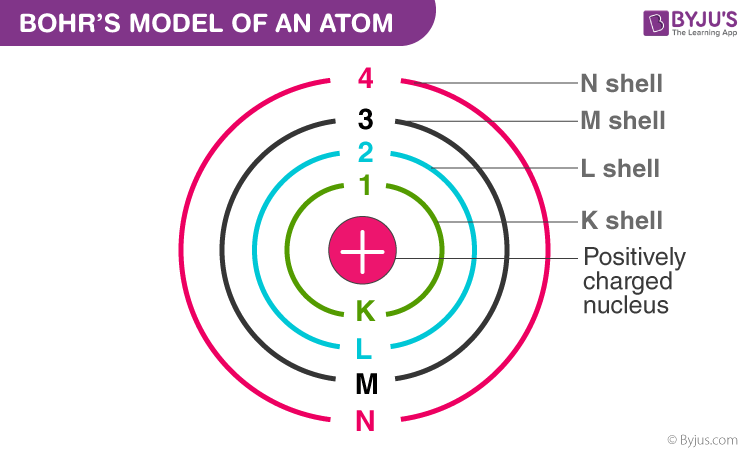
\includegraphics[width=0.75\linewidth]{atom.png}
    \caption{Structure of an atom}
\end{figure}
An atom of X element has Z number of protons, N number of neutrons [n(0)], and a mass (A) of Z+N. An element can be expressed as $\ch{^{A}_{Z}X}$ \par.
%-------------------------------------------------------------------------------------------------------------------------------------------------------------------------------------------------------------------------------------------------------------------------------------------------------------------------------------%
\section{Stability of atomic nuclei}
\begin{figure}
    \centering
    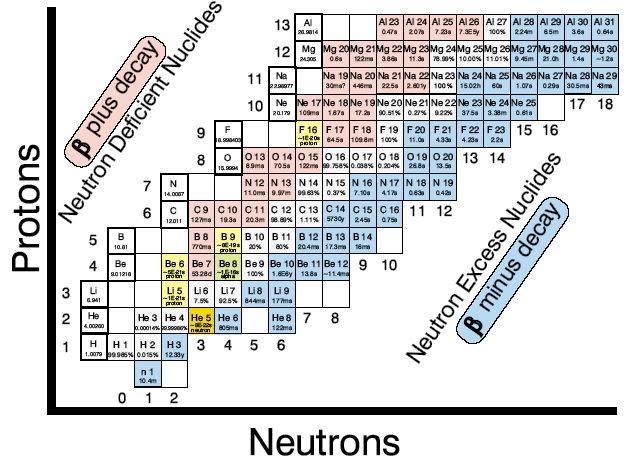
\includegraphics[width=0.75\linewidth]{chart_of_nucleides.png}
    \caption{Chart of Nucleides}
\end{figure}
%-------------------------------------------------------------------------------------------------------------------------------------------------------------------------------------------------------------------------------------------------------------------------------------------------------------------------------------%
\section{Radionucleides}
Some elements only exist as a radionucleide. Some elements exist with a very minute fraction of radioisotopes. There are also many artificial radionucleides.
%-------------------------------------------------------------------------------------------------------------------------------------------------------------------------------------------------------------------------------------------------------------------------------------------------------------------------------------%
\section{Activity and specific activity}
The nucleus of an unstable nucleide decays spontaneously to another nucleide (disintegration). Not affected by temperature, pressure, etc. Which nucleus will decay isn't predictable, but on average, it will decay. Activity is the decrease in radioactive nuclei per time.
\[A(t) := \frac{dN(t)}{dt}\]
The activity is expressed in Bq (1 disintegration per second). \\
Prefixes are used: k ($10^3$), M ($10^6$), G ($10^9$), T ($10^12$), m ($10^-3$), $\mu$ ($10^-6$), n ($10^-9$).
%-------------------------------------------------------------------------------------------------------------------------------------------------------------------------------------------------------------------------------------------------------------------------------------------------------------------------------------%
\section{Electromagnetic radiation}
Both a wave and a particle. The energy is expressed in J, or eV. $1\ eV = 1.6*10^{-19}\ J$. The binding energy of electrons on the outer shell is $\approx$ 30 eV. Photons and particles released are expressed in keV or MeV. X-rays are usually between 10 and 100 keV, while $\gamma$ radiation is usually between 100 and 1000 keV. 
%-------------------------------------------------------------------------------------------------------------------------------------------------------------------------------------------------------------------------------------------------------------------------------------------------------------------------------------%
\section{The radiation and the particles released during decay}
\subsection{$\alpha$ decay} Occurs when the nucleus is unstable, due to being too big. The parent atom $\ch{^{A}_{Z}X}$ gets split into a daughter atom $\ch{^{A-4}_{Z-2}Y}$ and an alpha particle $\ch{^{4}_{2}a}$.\\\\
\subsection{$\beta^{-}$ decay} Occurs when the nucleus is unstable, due to having an excess of neutrons. The parent atom $\ch{^{A}_{Z}X}$ gets split into a daughter atom $\ch{^{A}_{Z+1}Y}$, a beta particle $\ch{^{0}_{-1}e^{-}}$, and an anti-neutrino $\overline{v}_e$.\\\\
\subsection{$\beta^{+}$ decay} Occurs when the nucleus is unstable, due to having an excess of protons. The parent atom $\ch{^{A}_{Z}X}$ gets split into a daughter atom $\ch{^{A}_{Z+1}Y}$, a positron $\ch{^{0}_{+1}e^{+}}$, and a neutrino $v$. After a number of interactions, the positron $\beta{+}$ unites with an electron and converts its entire mass to energy. This annihilation produces 511 keV.\\\\
\subsection{Electron capture} The nucleus absorbs an electron from the electron cloud (usually from shell K -innermost). The parent atom $\ch{^{A}_{Z}X}$ absorbs an electron $\ch{^{0}_{-1}e^{-}}$, and gets split into a daughter atom $\ch{^{A}_{Z-1}Y}$, and a neutrino $v$.\\\\
\subsection{Gamma decay ($\gamma$)} Occurs when the atom is excited. The parent atom $\ch{^{A}_{Z}X*}$ gets excited and produces a daughter particle $\ch{^{A}_{Z}X}$ and a gamma ray $\gamma^{1}$. Internal conversion may occur (direct transfer of the energy of the nucleus to an electron).
\subsection{Internal conversion (IC)} Instead of $\gamma$ decay, internal conversion can occur. This is the the direct transfer of energy of the nucleus to an electron. The electron (conversion electron) is ejected from orbit with large energy, and can be detected as a $\beta^{-}$ particle, but with a sharply defined energy (unlike $\beta^{-}$, who share with neutrinos). Otherwise, can be considered a $\beta^{-}$ particle. This leaves a gap in the electron cloud, becoming unstable
\subsection{Follow-up processes: characteristic X-rays and Auger electrons} After the nucleus transfers energy to an electron or captures an electron, a vacancy is formed, filled by an electron a shell further away from the nucleus. The difference in binding energy causes the emission of characteristic X-ray spectrum (there's one emission per electron that descends = as many as electron shells there are). Due to this, other electrons may be ejected, known as Auger electrons.
%-------------------------------------------------------------------------------------------------------------------------------------------------------------------------------------------------------------------------------------------------------------------------------------------------------------------------------------%
\section{Parent-daughter relations}
After decay, the daughter nucleide may also be unstable. If the half-life is shorter, it's called ''ingrowth of activity'' (total activity grows). This must be taken into account.
%-------------------------------------------------------------------------------------------------------------------------------------------------------------------------------------------------------------------------------------------------------------------------------------------------------------------------------------%
\section{The time sequence in the decay processes}
An instable nucleide may have more than one decay process. Decay schemes explain graphically the decay. Parent level (top level), daughter level (bottom level), disintegration energy between them (Q). Increase in Z-value = right arrow; decrease in Z-value or EC = left arrow. 


\end{document}